\subsection{The Next-to-Minimal-Supersymmetric Standard Model}\label{sec:susy}
In supersymmetric theories, every SM particle has a \textit{superpartner} which differs in spin by $1/2$. In other words, every SM boson has a fermionic superpartner, and every SM fermion has a bosonic superpartner. Supersymmetric extensions of the SM are motivated by a solution to the hierarchy problem, an automatic unification of the running gauge couplings at a Grand Unified (GUT) scale $M_{\text{GUT}}$, and the introduction of a stable neutral particle which can be identified as a dark matter candidate~\cite{Ellwanger:2009dp}. 

In the Minimal Supersymmetric Standard Model (MSSM), there are two Higgs \SU{2}-doublets, $\Phi_1$ and $\Phi_2$, which lead to three neutral and two charged Higgs bosons~\cite{Fayet:1974pd,Fayet:1977yc}. An unattractive property of the MSSM is that the Lagrangian must contain a supersymmetric mass term for the Higgs doublets, which has to be of the order of the SUSY breaking scale, $M_{\text{SUSY}}$, for phenomenological reasons. Ideally, the electroweak scale generated by the Higgs vevs would depend only on $M_{\text{SUSY}}$, which would be the only remaining scale asking for an explanation as to why it is far below $M_{\text{GUT}}$ or the Planck scale $M_{\text{Planck}}$. This issue with the MSSM, denoted as the ``$\mu$-problem'', is rectified in the Next-to-Minimal Supersymmetric Standard Model (NMSSM)~\cite{Ellwanger:2009dp} and the solution requires the introduction of a singlet field, $S$. Models with this scalar structure are referred to as two-Higgs-doublet + singlet models (2HDM+S).

In 2DMH+S models, there are 3 CP-even and 2 CP-odd neutral scalars, and in the gauge eigenbasis these are denoted $H^{\text{SM}}$, $H^{\text{NSM}}$, $H^{\text{S}}$ and $A^{\text{NSM}}$, $A^{\text{S}}$ for the CP-even and CP-odd bosons respectively. The couplings of these states to SM particles are:
\begin{align*}
    H^{\text{SM}}(f_1,f_2,\mathrm{VV}) &= (g_{\text{SM}}, g_{\text{SM}}, g_{\text{SM}}), \\
    H^{\text{NSM}}(f_1,f_2,\mathrm{VV}) &= (g_{\text{SM}}/\tan{\beta}, -g_{\text{SM}}\tan{\beta}, 0), \\
    H^{\text{S}}(f_1,f_2,\mathrm{VV}) &= (0,0,0), \\
    A^{\text{NSM}}(f_1,f_2,\mathrm{VV}) &= (g_{\text{SM}}/\tan{\beta}, -g_{\text{SM}}\tan{\beta}, 0), \\
    A^{\text{S}}(f_1,f_2,\mathrm{VV}) &= (0,0,0)
\end{align*}
where $f_1$ ($f_2$) are SM fermions that couple to $\Phi_1$ ($\Phi_2$), $\mathrm{VV}$ corresponds to pairs of $\mathrm{W}$ or $\mathrm{Z}$ bosons, $g_{\text{SM}}$ is the coupling of a SM Higgs boson to such particles, and $\tan{\beta}$ is the ratio of vacuum expectation values: $\tan{\beta}=v_1/v_2$ where $v_1\equiv \langle \Phi_1 \rangle$ and  $v_2 \equiv \langle \Phi_2 \rangle$~\cite{Baum:2018zhf}.

The CP-even and CP-odd mass eigenstates obtained after mixing of gauge eigenstates are denoted $h_i=\{h_{125},H,h\}$ and $a_i=\{A,a\}$ respectively where $h_{125}$ is identified as the 125 GeV SM-like state observed at the LHC. The mass ordering is such that $m_H>m_h$ and $m_A>m_a$. In the alignment limit where $h_{125} = H^{\text{SM}}$, couplings for interactions involving $h_{125}h_{125}$ and one of the other scalars go to zero. On the other hand, couplings for $Hhh_{125}$ and $Aah_{125}$ are non-zero, which allows for so-called \textit{cascade decays}: $H\rightarrow h h_{125}$ and $A \rightarrow a h_{125}$. This motivates the \XYH search in \cref{chap:dihiggs} where \PX and \PY are new scalars, and \PH is the SM Higgs boson.

\subsubsection{$Y\rightarrow \gamma\gamma$ in the NMSSM at Low \mY}\label{sec:low_mass_in_NMSSM}

\begin{figure}
    \centering
    \inputtikz{Figures/Theory/SUSY/a_gamgam.tex}
    \caption[Feynman Diagram for a CP-Odd Higgs Boson Decaying to Two Photons Via a Chargino Loop]{Feynman diagram for the decay of the CP-odd Higgs boson, $a$, to two photons mediated by a chargino ($\chi^\pm$) loop.}\label{fig:a_gamgam}
   \end{figure}

If the lightest CP-odd Higgs in the mass basis, $a$, is very singlet-like, i.e.\ its main component is $A^S$, then its couplings to SM particles are heavily suppressed, and therefore, the typical hierarchy of Higgs decays: $bb, WW, \tau\tau, ZZ,\ldots$ becomes irrelevant. It is still possible for $a$ to decay to SM particles through loop interactions (see \cref{fig:a_gamgam}). The Higgs decay to two photons, which is suppressed in the SM, can now become the dominant decay mode for $a$, with a branching fraction up to 85\% depending on the theoretical scenario~\cite{King:2014xwa}. Since $a$ couples weakly to SM particles, its direct production, $pp \to a$ is also suppressed. The couplings of $a$ to BSM particles are however, not suppressed. Therefore, a search for $pp \rightarrow A \rightarrow a h_{125}$, where $a\to\gamma\gamma$, is uniquely placed to study this region of the NMSSM phase space. This motivates the inclusion of \Ygg in the \XYH search in \cref{chap:dihiggs}. 

In Ref.~\cite{Ellwanger:2022jtd}, maximally-allowed cross sections for this process are calculated given constraints from a set of relevant measurements. These cross sections are shown in \cref{fig:max_allowed_constraints}. If in the search for this process, we can set upper limits for the cross sections below the maximally-allowed, it means that our search will provide tighter constraints on the NMSSM than available at the time that Ref.~\cite{Ellwanger:2022jtd} was published (May 2022).

\begin{figure}[h]
    \centering
    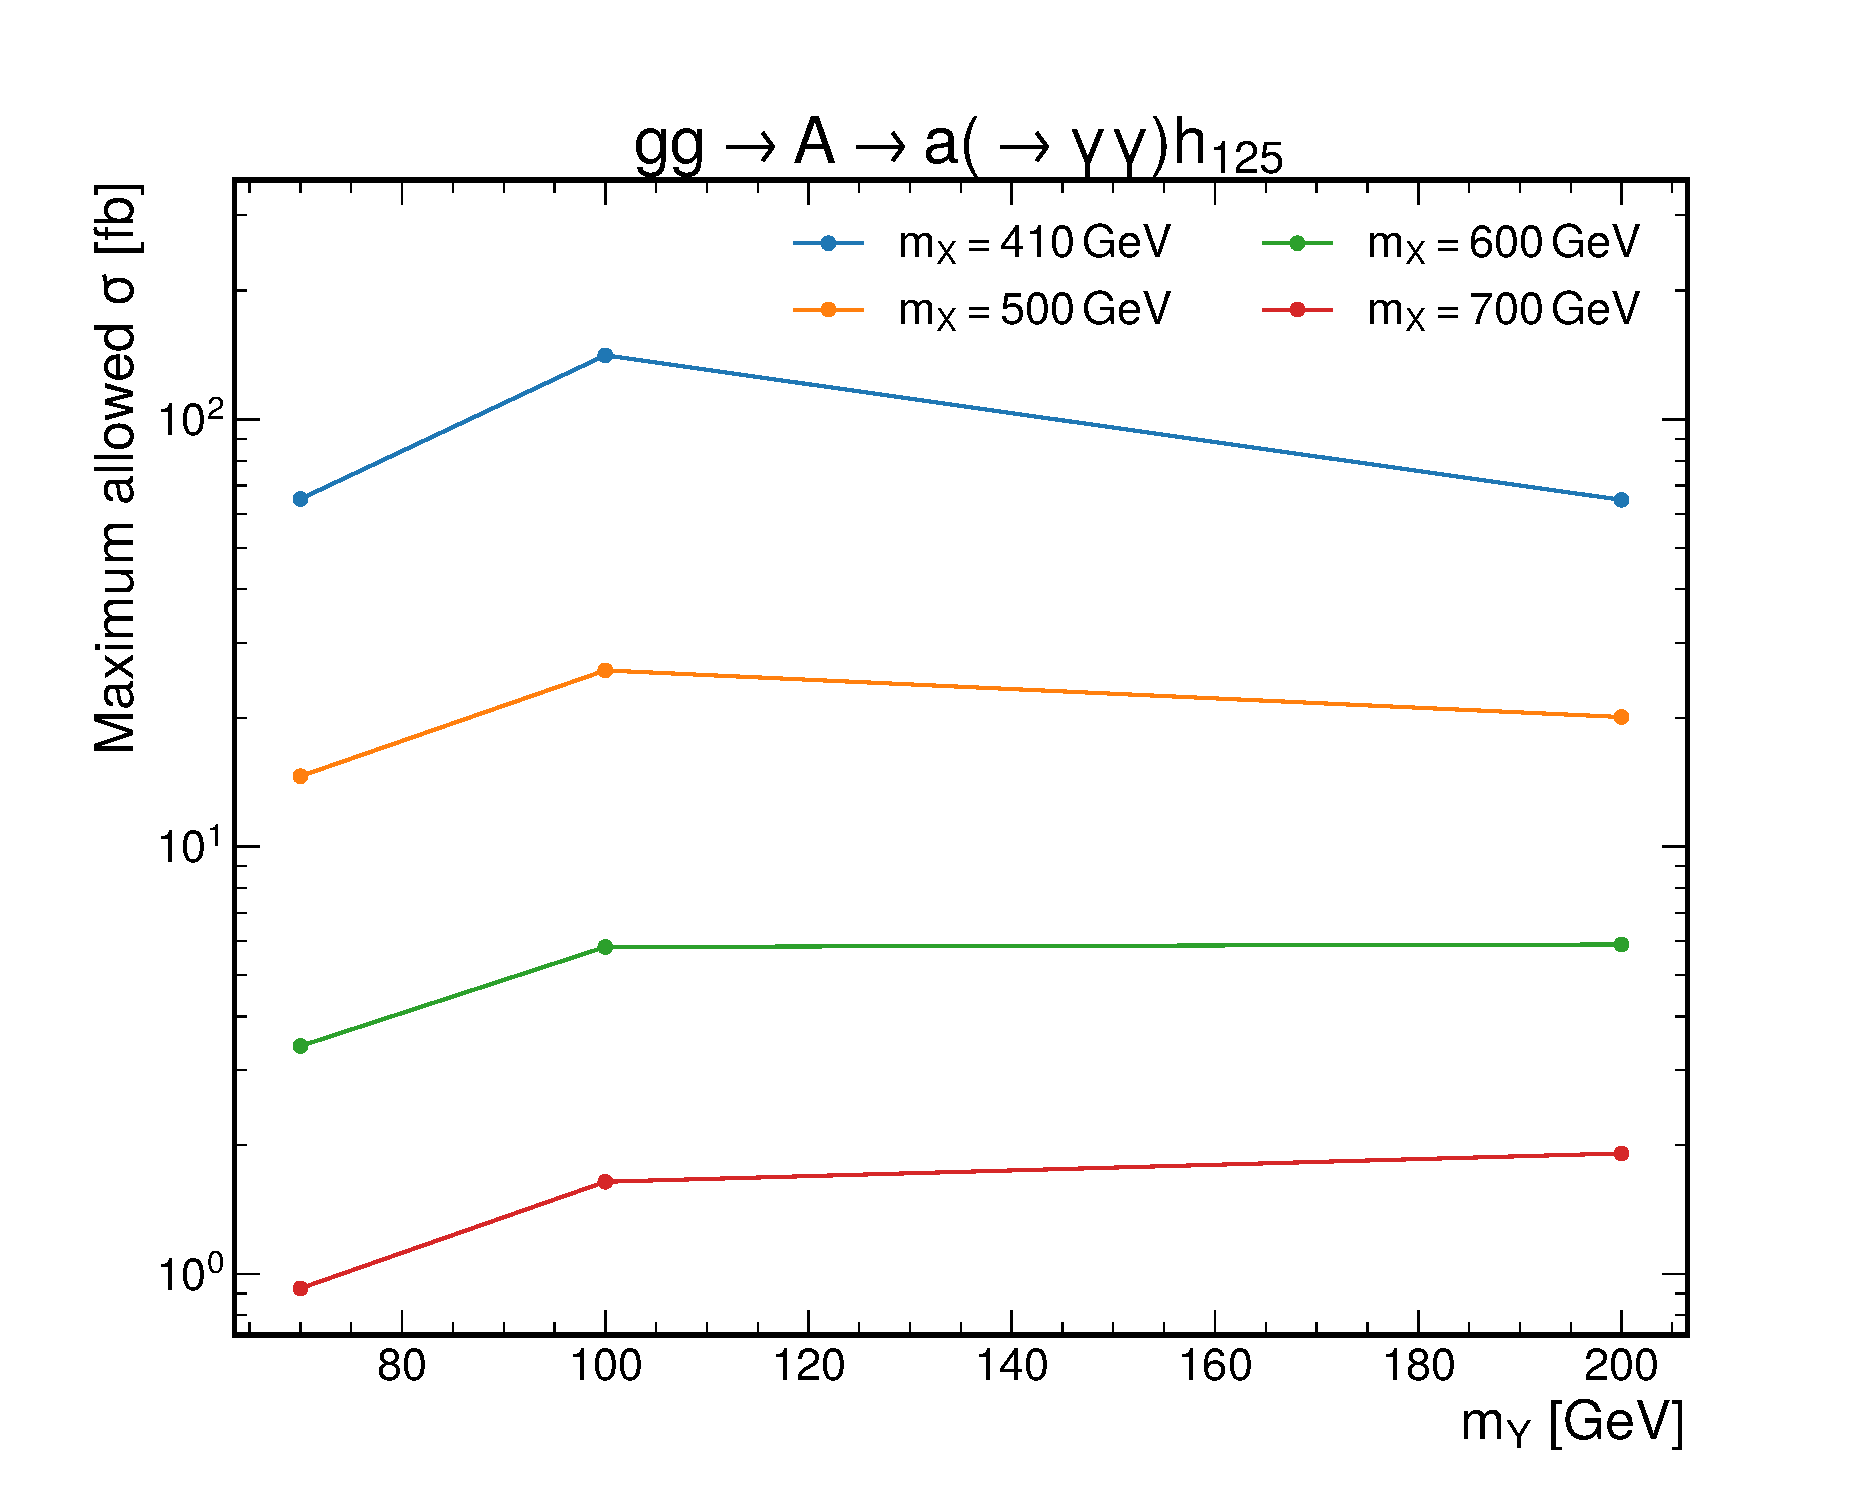
\includegraphics[width=0.7\textwidth]{Figures/Theory/SUSY/max_allowed_limits.pdf}
    \caption[Maximally-Allowed Cross Sections for $pp\rightarrow A \rightarrow H_{125}(\rightarrow\tau\tau)a(\rightarrow\gamma\gamma)$ in the NMSSM]{Maximally-allowed cross sections for $pp\rightarrow A \rightarrow h_{125}a(\rightarrow\gamma\gamma)$ in the NMSSM provided experimental constraints~\cite{Ellwanger:2022jtd}.}\label{fig:max_allowed_constraints}
\end{figure}